\section{Ajax}
\label{ch:ajax}

\subsection{Présentation}

AJAX (Asynchronous JavaScript And XML) est une architecture informatique permettant de construire des sites web dynamiques interactifs et des applications Web en se servant de différentes technologies présentées précédemment.

Ajax combine JavaScript, XML, CSS, le DOM et XMLHttpRequest afin d’améliorer la maniabilité et le confort d’utilisation des Applications Internet Riches (RIA).

Le terme Ajax a été introduit par Jesse James Garrett, le 18 février 2005, dans un article sur le site Web Adaptive Path. Ajax a créé une petite révolution dans les navigateurs.

En utilisant Ajax, le dialogue entre le navigateur et le serveur se déroule la plupart du temps de la manière suivante:

\begin{figure}[ht!]
\begin{center}
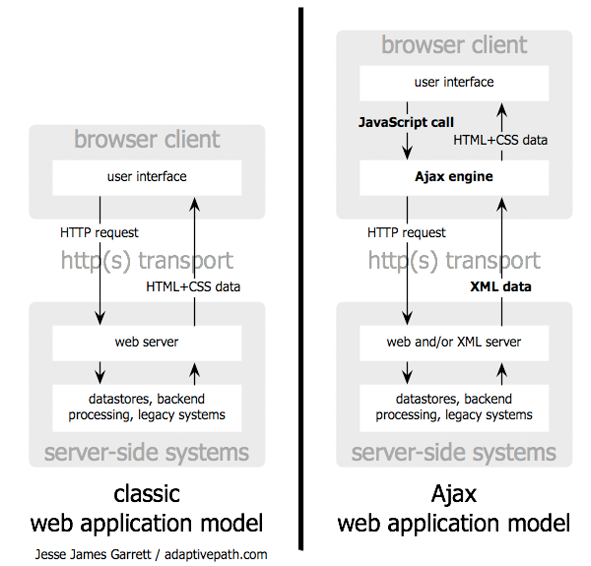
\includegraphics[scale=0.6]{img/ajax.png}
\caption{Graphique technologie ajax}
\end{center}
\end{figure}


Les échanges de données entre le client et le serveur peuvent utiliser d’autres formats notamment le format JSON.

Ajax a permis à JavaScript de gagner en popularité et de ne plus être le vilain petit canard des langages de programmation. Ainsi avec AJAX JavaScript n’est plus un langage qui se contente d'afficher des popup intempestives ou de vérifier des formulaires.

Google a marqué les esprits avec Google Maps. Maps n’aurait jamais pu exister sans Ajax. L’utilisation de JavaScript par Google a permis à JavaScript de montrer son potentiel. Depuis JavaScript s’est désinhibé, et de véritables logiciels sont apparus dans nos navigateurs.

Google est un très gros consommateurs de JavaScript notamment avec Drive ou Gmail.

JavaScript est donc passé du petit langage d’agrément pour pages web à un langage de développement d’applications réseau supporté par tout les navigateurs quel que soit le système d’exploitation. Et le navigateur, pour un grand nombre d’utilisateurs, est la porte d’entrée de l’ordinateur et du réseau.

Avant AJAX: la page web est le support pour de petites applications JavaScript, le plus souvent d’agrément et facultatives pour utiliser le contenu.

Avec AJAX: JavaScript deviens le cœur du site. Il génère du contenu HTML dont il a la maîtrise. Avec un autre langage coté serveur, JavaScript coté client s’appuie sur le moteur graphique du navigateur pour générer l’interface de l’application, plus pratique que n’importe quel “toolkit”.

Cette mutation a pris du temps. Le navigateur est passé d’un logiciel pour consulter des pages web à un logiciel permettant d’exécuter d’autres logiciels (en somme comme un système d’exploitation).

Ajax est donc plébiscité parce qu’il donne naissance à des applications inédites accessible à travers notre navigateur. Avec AJAX une application comme Google Earth pourrait aussi bien exister de façon autonome.

Malgré toutes ces avancées, JavaScript était encore confronté a des obstacles majeurs qui ont freiné son adoption.

JavaScript étant exécuté par le navigateur, ses performances de l’époque étaient extrêmement faibles. Actuellement la bataille des navigateurs se fait sur de meilleurs support tels que HTML5/CSS3 mais aussi sur les performances des moteurs JavaScript. L’arrivée de Google Chrome et des énormes besoins de Google en performances JavaScript ont poussé tout les acteurs du marché à améliorer les moteurs pour toujours plus de performances.

Le second problème de JavaScript est l'exécution du script par le moteur. En fonction du navigateur utilisé, le code JavaScript doit être différent, chaque éditeur étant libre d’intégrer JavaScript comme il le souhaite. Ainsi un code JavaScript peut fonctionner correctement sur Firefox ou Chrome mais pas sur Internet Explorer.

Le Javascript est aussi un langage qui nécessite des efforts importants et dont le développement en AJAX pur peut être extrêmement coûteux.

Afin de résoudre ce problème de développement, John Resig à sortie un framework révolutionnant la façon d’écrire du code JavaScript. Le nom de ce framework: jQuery.

